\documentclass[oneside,final,12pt]{article}
\usepackage[utf8]{inputenc}
\usepackage[russianb]{babel}
\usepackage{vmargin}
\usepackage{amsmath}
\usepackage{amsfonts}
\usepackage{amssymb}
\usepackage{amsthm}
\usepackage[matrix,arrow,curve]{xy}
\usepackage{graphicx}
\usepackage{subfig}
\setpapersize{A4}
\setmarginsrb{2cm}{1.5cm}{1cm}{1.5cm}{0pt}{0mm}{0pt}{13mm}
\usepackage{indentfirst}
\sloppy

\DeclareMathOperator{\tr}{tr}

\newcommand*\Rn  [1]{\mathbb{R}^{#1}}
\newcommand*\Za {\mathbb{Z}}
\newcommand*\Na {\mathbb{N}}

\renewcommand*\leq{\leqslant}
\newcommand*\eps{\varepsilon}
\newcommand*\steq{\Leftrightarrow}

\newcommand*\valat[2]{\left.#1\right|_{#2}}
\newcommand*\abs[1]{|#1|}
\newcommand*\norm[2]{\|#1\|_{#2}}
\newcommand*\segm[2]{[#1,#2]}
\newcommand*\inter[2]{(#1,#2)}
\newcommand*\scprod[2]{\bigl\langle #1 , #2 \bigl\rangle}
\newcommand*\point[2]{\begin{pmatrix} #1 \\ #2 \end{pmatrix}}

\newcommand*\picsize{0.5\textwidth}
\newcommand*\bigpicsize{0.7\textwidth}
\newcommand*\subpicsize{0.45\textwidth}
\newcommand*\subtripicsize{0.3\textwidth}
\newcommand*\picpath{pictures/}

\theoremstyle{plain}
\newtheorem*{theorem}{Теорема}
\theoremstyle{remark}
\newtheorem*{remark}{Замечание}
\theoremstyle{definition}
\newtheorem{definition}{Определение}
\theoremstyle{plain}
\newtheorem{statement}{Утверждение}

\begin{document}
	\begin{titlepage}
		\begin{centering}
			\includegraphics[width=0.5\textwidth]{\picpath msu.png}\\
			{\scshape Московский государственный университет имени М.~В.~Ломоносова}\\
			Факультет вычислительной математики и кибернетики\\
			Кафедра системного анализа\\
			\vfill
			{\LARGE Курсовая работа. Часть 2}\\
			\vspace{1cm}
			{\Huge\bfseries "<Исследование нелинейной динамической системы на плоскости">\\}
		\end{centering}
		\vspace{1cm}
		\begin{flushright}
			\begin{large}
				{\itshape Студент 315 группы\\}
				А.~А.~Владимиров\\
				\vspace{5mm}
				{\itshape Научный руководитель\\}
				Д.~А.~Алимов\\
			\end{large}
		\end{flushright}
		\vfill
		\begin{centering}
			Москва, 2021\\ 
		\end{centering}
	\newpage
	\end{titlepage}
	\setcounter{page}{2}
	
	\tableofcontents

	\section{Постановка задачи}
		Дана система обыкновенных дифференциальных уравнений
		\begin{equation}\label{odu} \left\{ \begin{aligned}
			\dot x & = ax(K-x) - \frac{bxy}{1+Ax},\\
			\dot y & = -cy + \frac{dxy}{1+Ax},	\\
		\end{aligned}\right. \end{equation}
где \((x,y) \in \Rn{2}_+\)~--- фазовые переменные; \(a, b, c, d, K, A\)~--- положительные параметры.
		
		Динамическая система, задаваемая уравнениями \eqref{odu}, суть есть модель "<хищник--жертва"> Холлинга\footnote{\cite{DSMB} п. 7.2.}. Здесь \(x\) и \(y\)~--- численности жертв и хищников соответственно. 

		\bigskip
		Следуя \cite{DSMB}, перезапишем систему \eqref{odu} в более общем виде и, вкратце, поясним биологический смысл входящих в запись системы компонент
		\[		\left\{ \begin{aligned}
				\dot x & = A(x) - B(x,y),\\
				\dot y & = -C(y) + D(x,y).	\\
				\end{aligned}\right. \]
		
		{\newcommand*\eqodu{\stackrel{\eqref{odu}}{=}}
		\(A(x)\)~--- функция, описывающая размножение жертв при отсутствии хищников.  В системе \eqref{odu} \(A(x) \eqodu ax(K-x) = aKx(1 - \frac{x}{K})\)~--- логистическое уравнение, учитывающее фактор внутривидовой конкуренции жертв.\par
 		\(C(y)\)~--- описывает вымирание хищников при отсутствии жертв. \(C(y) \eqodu cy\)~--- классическая модель Мальтуса экспоненциального роста (в нашем случае вырождения) изолированной популяции.\par
		\(B(x,y)\)~--- описывает выедание жертв хищниками. \(B(x,y) = B_1(x)B_2(y).\)
			\begin{itemize}
				\item[\(B_1(x)\)~---] трофическая функция хищника. \(B_1(x) \eqodu \frac{x}{1+Ax}\)~--- модель Моро, отражающая явление насыщения хищника.
				\item[\(B_2(y)\)~---] зависимость скорости выедания жертвы от плотности популяции хищника. \(B_2(y) \eqodu by\)~--- линейная функция, т.е. фактор конкуренции хищников за жертв исключен из рассмотрения.
			\end{itemize}
		\(D(x,y)\)~--- эффективность потребления жертв хищниками. \(D(x,y) = D_1(x)D_2(y).\) В силу обыкновенно принимаемого в модели Лотки--Вольтерры предположения о постоянном коэффициенте переработки хищником пищи в собственную биомассу \(D_1(x) \eqodu B_1(x)\), \(D_2(y) \eqodu dy\).
		}

		\bigskip
		Требуется провести качественный анализ системы \eqref{odu} и дать биологическую интерпретацию полученным результатам.

	\section{Переход к безразмерным переменным}
		{\newcommand*\ag{\alpha}
		\newcommand*\bg{\beta}

		Перед дальнейшим исследованием системы попробуем сократить колчиество параметров линейной заменой координат. Пусть
		\begin{equation}\label{xy_subs}
			\left\{ \begin{aligned}
				x & = \ag u,\\
				y & = \bg v,\\
			\end{aligned}\right. 
			\quad \ag > 0, \: \bg > 0,
		\end{equation}
тогда
		\[\left\{ \begin{aligned}
			\ag\dot u & = a\ag u(K-\ag u) - \frac{b\ag u \bg v}{1+A \ag u},\\
			\bg\dot v & = -c\bg v + \frac{d \ag u \bg v}{1+A \ag u},	\\
		\end{aligned}\right. \]
что равносильно
		\[\left\{ \begin{aligned}
			\dot u & = a u(K-\ag u) - \frac{b u \bg v}{1+A \ag u},\\
			\dot v & = -c v + \frac{d \ag u v}{1+A \ag u}.	\\
		\end{aligned}\right. \]
Пусть 
		\begin{equation}\label{albe_def}
			\ag = K,\: \bg = b^{-1},
		\end{equation}
 тогда
		\[\left\{ \begin{aligned}
			\dot u & = aKu(1-u) - \frac{uv}{1+AK u},\\
			\dot v & = -cv + \frac{dK u v}{1+AK u}.	\\
		\end{aligned}\right. \]
В качестве новых параметров положим
		\begin{equation}\label{efgh_def}
			e = aK,\: f = c,\: g = AK,\: h = dK.
		\end{equation}

	Таким образом, после замены \eqref{xy_subs}, \eqref{albe_def} и переобозначений \eqref{efgh_def} получим систему, имеющую четыре параметра,
		\begin{equation}\label{odu_subs}
			\left\{ \begin{aligned}
				\dot u & = eu(1-u) - \frac{uv}{1+g u},\\
				\dot v & = -fv + \frac{h u v}{1+g u}.	\\
			\end{aligned}\right.
		\end{equation}

	Изучение моделей с числом параметров больше двух довольно трудоемкая, а порой практически не выполнимая задача\footnote{\cite{DSMB} п. 5.7.}, поэтому в рамках данной работы будем пологать параметры \(f\) и \(g\) фиксированными и равными, например, единице.
	Таким образом, нам предстоит исследоавать динамику упрощенной системы 
		\begin{equation}\label{odu_simple_subs}
			\left\{ \begin{aligned}
				\dot u & = eu(1-u) - \frac{uv}{1+u},\\
				\dot v & = -v        + \frac{huv}{1+u}.	\\
			\end{aligned}\right.
		\end{equation}

		}

	\section{Неподвижные точки}
		Система \eqref{odu_simple_subs} имеет три неподвижных точки\footnote{Напомним, что как и в предыдущей части работы подавляющее большинство вычислений выполнено посредством пакета символьной компьютерной алгебры \texttt{MatLab}. С ходом этих вычислений можно ознакомиться в приложенном \texttt{.mlx} файле.}
		\[\point{0}{0}, \quad \point{1}{0}, \quad \point{u^*}{v^*},\]
где \(\displaystyle{u^* =\frac{1}{h-1},\: v^* = \frac{eh(h-2)}{(h-1)^2}}\). В дальнейшем будем называть их \(a_1\), \(a_2\) и \(a_3\) соответственно. 

	\bigskip
		Первые две точки тривиальны: \(a_1\) соотвутствует вымиранию обоих видов, \(a_2\)~--- вымиранию хищников, при некоторой установившейся численности жертв. Больший интерес представляет третья неподвижная точка. Точка \(a_3\) отвечает состоянию экологического равновесия~--- стабильному сосуществованию обоих видов.
	
	\bigskip
		Для установления типа каждой неподвижной точки, воспользуемся известным приемом,\footnote{см. \cite{DSMB} п. 4.2.} позволяющим узнать характер гиперболического (негиперболические мы рассматривать не будем) положения равновесия на плоскости. Для этого достаточно информации о \(\tr J\) и \(\det J\)~--- следе и определителе матрицы Якоби системы дифференциальных уравнений.
		
		Итак, каждому типу равновесия соответствует область значений \(\tr J\) и \(\det J\), изображенная на рис. \ref{stabilities}. \(I\)~--- устойчивые фокусы, \(II\)~--- неустойчивые фокусы, \(III\)~--- неустойчивые узлы, \(IV\)~--- устойчивые узлы, \(V\), \(VI\)~--- седла.

		\begin{figure}[!h]
			\centering
			\includegraphics[width=\picsize]{\picpath stabilities}
			\caption{Устойчивость положений равновесия, в зависимости от \(\tr J\) и \(\det J\). Кривая на графике: \(4\det J = \tr^2 J\).} \label{stabilities}
		\end{figure}

		Таким образом, для каждой неподвижной точки требуется выяснить в какой области в зависимости от параметров лежат соответствующие значения \(\tr J\) и \(\det J\). 

		Приведем диаграммы, показывающие, где относительно каждой  из кривых (\(\tr J = 0\), \(\det J = 0\), \(4\det J = \tr^2 J\)) лежат значения \(\tr J\) и \(\det J\), в зависимости от параметров \(e\) и \(h\). На их основании построены разбиения пространства параметров на области \(I\)--\(VI\).
	
	\newpage
	\paragraph{Первая точка} (рис. \ref{stp1_diagrams}, \ref{stp1_portrait}) является седловой вне зависимости от значений параметров и не представляет интереса.

		\begin{figure}[!h]
			\centering
			\subfloat[\centering ] 
			{{\includegraphics[width=\subpicsize]{\picpath stp1/trJ} }}
			\:
			\subfloat[\centering ]
			{{\includegraphics[width=\subpicsize]{\picpath stp1/detJ} }}
			\:
			\subfloat[\centering ]
			{{\includegraphics[width=\subpicsize]{\picpath stp1/trJdetJ} }}
			\caption{Диаграммы первой точки.}\label{stp1_diagrams}
		\end{figure}

		\begin{figure}[!h]
			\centering
			\includegraphics[width=\picsize]{\picpath stp1/stability_portrait}
			\caption{Параметрический портрет первого положения равновесия.} \label{stp1_portrait}
		\end{figure}

	\newpage
	\paragraph{Вторая точка} (рис. \ref{stp2_diagrams}, \ref{stp2_portrait})~--- устойчивый узел при \(h < 2\), седло при \(h > 2\).

		\begin{figure}[!h]
			\centering
			\subfloat[\centering ] 
			{{\includegraphics[width=\subpicsize]{\picpath stp2/trJ} }}
			\:
			\subfloat[\centering ]
			{{\includegraphics[width=\subpicsize]{\picpath stp2/detJ} }}
			\:
			\subfloat[\centering ]
			{{\includegraphics[width=\subpicsize]{\picpath stp2/trJdetJ} }}
			\caption{Диаграммы второй точки}\label{stp2_diagrams}
		\end{figure}

		\begin{figure}[!h]
			\centering
			\includegraphics[width=\picsize]{\picpath stp2/stability_portrait}
			\caption{Параметрический портрет второго положения равновесия.} \label{stp2_portrait}
		\end{figure}

	\newpage
	\paragraph{Третья точка} (рис. \ref{stp3_diagrams}, \ref{stp3_portrait}), как было отмечено выше, нетривиальна
		\[ \left(\frac{1}{h-1}, \frac{eh(h-2)}{(h-1)^2}\right). \] 
Нетрудно заметить, что при \(h < 2\) точка \(a_3\) не принадлежит фазовому пространству \(\Rn{2}_+\) (этот факт отражен на диаграмме знаком "<---">).  При \(h > 2\) возможны два варианта:
		\[\begin{aligned}
			&a_3 \text{~--- устойчивый узел},   &\text{при}\quad 2 < h < \sqrt{\frac{\sqrt{4e+1}+1}{2}} + 1, \\
			&a_3 \text{~--- устойчивый фокус}, &\text{при}\quad h > \sqrt{\frac{\sqrt{4e+1}+1}{2}} + 1. 
		\end{aligned}\]

		\begin{figure}[!h]
			\centering
			\subfloat[\centering ] 
			{{\includegraphics[width=\subpicsize]{\picpath stp3/trJ} }}
			\:
			\subfloat[\centering ]
			{{\includegraphics[width=\subpicsize]{\picpath stp3/detJ} }}
			\:
			\subfloat[\centering ]
			{{\includegraphics[width=\subpicsize]{\picpath stp3/trJdetJ} }}
			\caption{Диаграммы третьей точки.}\label{stp3_diagrams}
		\end{figure}

		Теперь у нас достаточно информации чтобы построить параметрический портрет системы.
	\newpage

		\begin{figure}[!t]
			\centering
			\includegraphics[width=\picsize]{\picpath stp3/stability_portrait}
			\caption{Параметрический портрет третьего положения равновесия.} \label{stp3_portrait}
		\end{figure}

\section{Параметрический портрет системы}
имеет следующий вид

		\begin{figure}[!h]
			\centering
			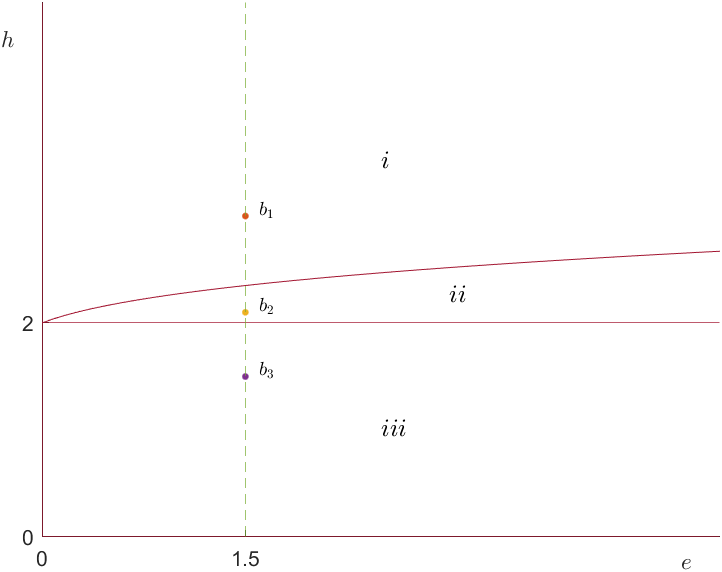
\includegraphics[width=\picsize]{\picpath phase_portraits/parametric_portrait}
			\caption{Параметрический портрет системы.} \label{parametric_portrait}
		\end{figure}
	
		Типы точек \(a_2\) и \(a_3\) (\(a_1\)--- всегда седло) 
		\begin{itemize}
			\item[] область \(i\): \(a_2\)~--- седло, \(a_3\)~--- устойчивый фокус;
			\item[] область \(ii\): \(a_2\)~--- седло, \(a_3\)~--- устойчивый узел;
			\item[] область \(iii\): \(a_2\)~--- устойчивый узел, \(a_3\)~--- не лежит в фазовой плоскости.
		\end{itemize}

		Двигаясь по прямой \(e = 1.5\) в направлении от точки \(b_1\) к точке \(b_3\), проследим эволюцию равновесия \(a_3\), и, попутно построим фазовые портреты системы в каждой из областей \(i\)--\(iii\).

		\bigskip
		Сперва напомним, что \(e = aK\), где \(aK\) можно интерпретировать, как скорость роста популяции жертв. Параметр \(h = dK\), характеризует совместное поведение величин \(d\)~--- эффективности потребления жертв хищниками и \(K\)~--- потенциальной емкости экологической системы относительно жертв (предельный размер популяции)\footnote{см. модель роста популяции, описываемую логистическим уравнением \cite{DSMB} п. 1.3. и \mbox{модель Холлинга \cite{DSMB} п. 5.6.}}. Исходные переменные \(x\) и \(y\) выражаются через \(u\) и \(v\) как \(x = Ku\), \(y = b^{-1}v\), откуда неподвижная токчка \(a_2 = (1,0)\) в исходных координатах имеет вид \((K,0)\).
		
		\bigskip
		Итак, в области \(i\) система \eqref{odu_simple_subs} имеет единственное положение устойчивого равновесия~--- фокус \(a_3\) (см. рис. \ref{phase_portrait_i}). Точка \(a_3\) соответствует состоянию экологического равновесия, к которому спиралевидно стремятся траектории системы. По всей видимости, \(a_3\) является глобальным аттрактором, а потому при любых (кроме, очевидно, нулевых) начальных размерах популяций ни одна из них не вырождается и обе колебательным образом стремятся к некоторой предельной численности.

		\begin{figure}[!h]
			\centering
			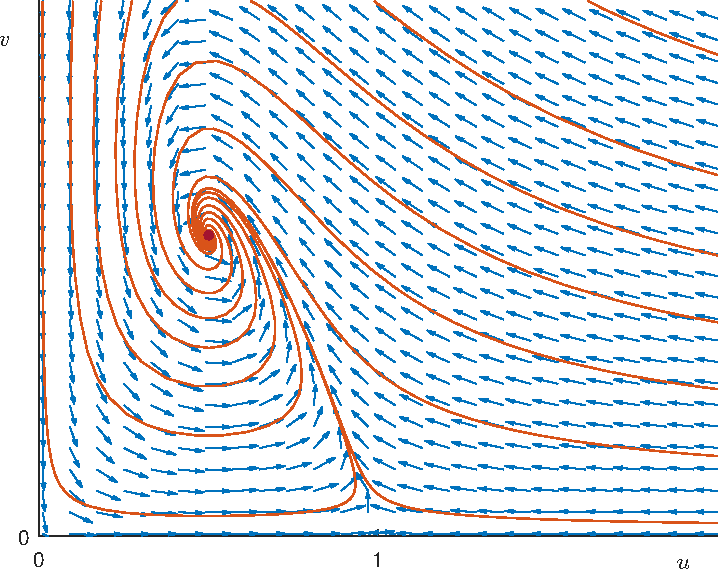
\includegraphics[width=\picsize]{\picpath phase_portraits/i}
			\caption{Фазовый портрет \(i\).} \label{phase_portrait_i}
		\end{figure}

		После перехода границы с областью \(ii\) \(a_3\) становится устойчивым узлом (рис. \ref{phase_portrait_ii}).

		\begin{figure}[!h]
			\centering
			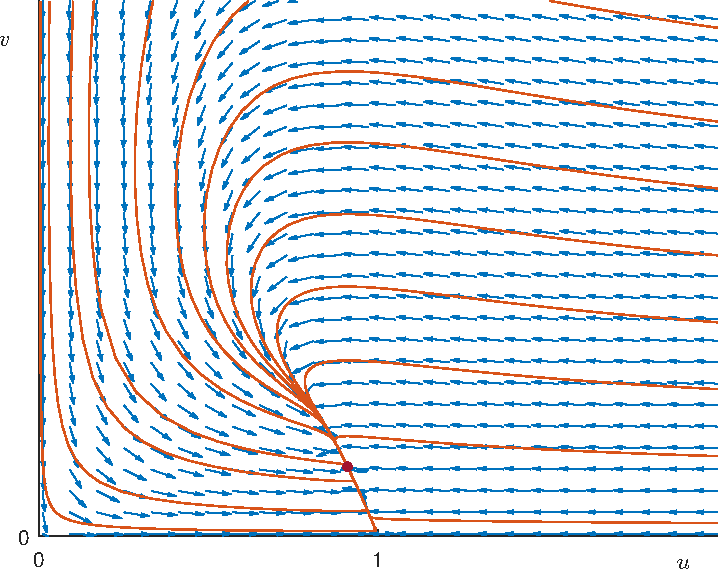
\includegraphics[width=\picsize]{\picpath phase_portraits/ii}
			\caption{Фазовый портрет \(ii\).} \label{phase_portrait_ii}
		\end{figure}

Поведение численности популяций в области \(i\) и \(ii\) вполне аналогично, за исключением того, что в случае \(ii\), в отличие от \(i\), траектории стремятся к положению равновесия "<напрямую">, a не колебательным образом.

		Наконец, на общей границе областей \(ii\) и \(iii\) точка \(a_3\) сливается c \(a_2\). В области \(iii\) единственным глобальным аттрактором является \(a_2\) (рис. \ref{phase_portrait_iii}). Экологическое равновесие системы становится невозможным: какими бы ни были начальные величины популяций, популяция хищников рано или поздно выродится, в то время как популяция жертв будет стабильно приближаться к своему потенциально возможному максимуму. 

		\begin{figure}[!h]
			\centering
			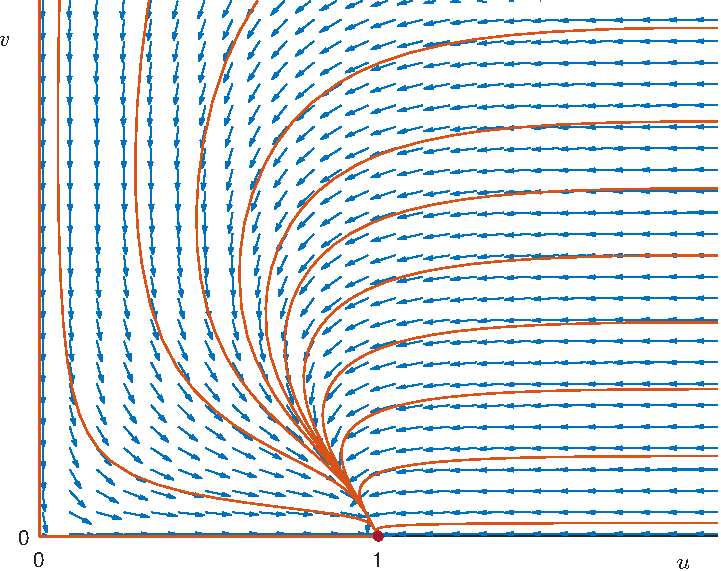
\includegraphics[width=\picsize]{\picpath phase_portraits/iii}
			\caption{Фазовый портрет \(iii\).} \label{phase_portrait_iii}
		\end{figure}
	
		Итак, мы проследили за изменением фазового портрета системы в зависимости от \(h\) при фиксированном \(e\). Приведем некоторые наблюдения. 

		Первое. Параметр \(e\) влияет лишь на размер инетрвала \(2 < h < \sqrt{\frac{\sqrt{4e+1}+1}{2}} + 1\) на котором \(a_3\) является узлом, что нам представляется несущественным, а потому зависимость системы от \(e\) мы опустим. 

		Второе. Положение равновесия \(a_3\) (если рассматривать \(a_2\) как выродившуюся при \(h<2\) точку \(a_3\)) в сущности целиком определяет фазовый портрет системы.
		
		\bigskip
		Отсюда вывод: поведение системы определяется зависимостью \(a_3\) от \(h\). Эта зависимость заключена в нескольких пунктах:
		\begin{itemize}
			\item При уменьшении \(h\) точка \(a_3\) сдвигается вниз и вправо на фазовой плоскости.
			\item При \(h < 2\) точка \(a_3\) вырождается в \(a_2 = (1,0)\).
			\item \emph{Вне зависимости} от \(h\) точка \(a_3\) устойчива.
		\end{itemize}

		Учитывая что \(h = dK\), полученный нами результат вполне согласуется с интуитивным пониманием биологического смысла поведения системы \eqref{odu}:
		\begin{itemize}
			\item При совокупном уменьшении параметров \(d\) и \(K\), т.е. эффективности потребления хищниками жертв и предельного числа жертв в популяции, количество\footnote{Имеется ввиду "<предельное"> количество, т.е. приблизительно установишееся за большой промежуток времени.} хищников уменьшается, а жертв увеличивается.
			\item Если параметры \(d\) и \(K\), уменьшить достаточно сильно (так, что они окажутся меньше некоторого граничного значения), то хищники вымрут, а жертвы достигнут своей максимально возможной численности.
			\item Система рано или поздно придет к состоянию экологического равновесия (при достаточно больших \(d\) и \(K\)), или вырождения (при достаточно малых \(d\) и \(K\)).
		\end{itemize}

		\paragraph{Замечание (о предельном цикле)}  Имеются основания пологать, что в рассматриваемой системе не возникает предельных циклов. Действительно, по физическим соображеням (на фазовой плоскости всегда существует ровно один сток, и ни одного истока), дивергенция векторного поля уравнения \eqref{odu_simple_subs} всюду не превосходит нуля. Следовательно, по критерию Бендиксона в системе \eqref{odu_simple_subs} предельных циклов нет.

	\bigskip
	\bigskip
	\bigskip
	\begin{thebibliography}{0}
		\bibitem{DSMB} Братусь~А.~С., Новожилов~А.~С., Платонов~А.~П.
			\emph{Динамические системы и модели биологии}. М.: ФИЗМАТЛИТ, 2010.
		\bibitem{KURS} Алимов~Д.~А. кафедральный курс 
			\emph{Динамические системы и биоматематика}, 2021.
	\end{thebibliography}

\end{document}